\documentclass[tikz,border=6pt]{standalone}
\usepackage{tikz}
\usetikzlibrary{patterns,arrows.meta,calc,decorations.markings,positioning}
\definecolor{linkblue}{RGB}{22,53,93}
\definecolor{loopsideroute}{RGB}{28,79,114}
\definecolor{loopsidefill}{RGB}{226,240,246}
\definecolor{gatecore}{RGB}{30,106,79}
\definecolor{gatetube}{RGB}{236,246,240}
\definecolor{gatechamber}{RGB}{235,242,252}
\definecolor{gatehigh}{RGB}{250,226,211}
\definecolor{gatepath}{RGB}{29,75,132}
\begin{document}
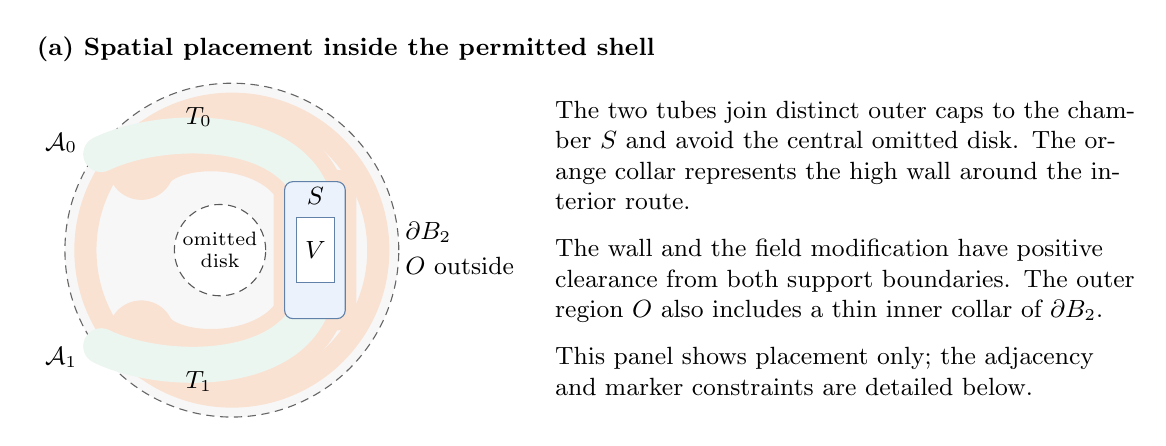
\begin{tikzpicture}[x=1cm,y=1cm,font=\small,
  cheap/.style={draw=gatetube,line width=13pt,line cap=round,line join=round},
  wall/.style={draw=gatehigh,line width=24pt,line cap=round,line join=round}]
  \node[anchor=west,font=\small\bfseries] at (0,4.90)
    {(a) Spatial placement inside the permitted shell};
  \fill[black!3] (2.60,2.35) circle (2.12);
  \draw[black!60,densely dashed] (2.60,2.35) circle (2.12);
  \draw[gatehigh,line width=8pt] (2.60,2.35) circle (1.86);
  \draw[wall] (1.45,3.41) .. controls (1.70,3.94) and (3.37,3.97) .. (3.65,2.96);
  \draw[wall] (1.45,1.29) .. controls (1.70,.76) and (3.37,.73) .. (3.65,1.74);
  \filldraw[fill=gatehigh,draw=none,rounded corners=7pt]
    (3.13,1.33) rectangle (4.18,3.37);
  \draw[cheap] (.94,3.57) .. controls (1.70,3.94) and (3.37,3.97) .. (3.65,2.96);
  \draw[cheap] (.94,1.13) .. controls (1.70,.76) and (3.37,.73) .. (3.65,1.74);
  \filldraw[fill=gatechamber,draw=gatepath!70,rounded corners=3pt]
    (3.27,1.48) rectangle (4.04,3.22);
  \filldraw[fill=white,draw=gatepath!70]
    (3.42,1.94) rectangle (3.90,2.76);
  \node at (3.66,2.35) {$V$};
  \node at (3.66,3.04) {$S$};
  \filldraw[fill=white,draw=black!65,densely dashed]
    (2.45,2.35) circle (.58);
  \node[align=center,font=\scriptsize] at (2.45,2.35)
    {omitted\\disk};
  \node[anchor=east] at (.76,3.71) {$\mathcal A_0$};
  \node[anchor=east] at (.76,.99) {$\mathcal A_1$};
  \node at (2.18,4.04) {$T_0$};
  \node at (2.18,.68) {$T_1$};
  \node[anchor=west] at (4.68,2.58) {$\partial B_2$};
  \node[anchor=west] at (4.68,2.15) {$O$ outside};
  \node[anchor=north west,align=left,text width=7.4cm,inner sep=0pt]
    at (6.70,4.25) {The two tubes join distinct outer caps to the
      chamber $S$ and avoid the central omitted disk.  The orange
      collar represents the high wall around the interior route.
      \par\medskip
      The wall and the field modification have positive clearance
      from both support boundaries.  The outer region $O$ also
      includes a thin inner collar of $\partial B_2$.
      \par\medskip
      This panel shows placement only; the adjacency and marker
      constraints are detailed below.};
\end{tikzpicture}
\end{document}
